\documentclass[sigconf,anonymous,review]{acmart}
\usepackage{amsmath,booktabs}
\usepackage{pgfplots}
\pgfplotsset{compat=1.18}
\setcopyright{none}
\settopmatter{printacmref=false,printccs=false,printfolios=true}
\acmConference[Research draft]{Internal research draft; not submitted}{October 2026}{Local artifact}
\acmYear{2026}
\title{Evaluating Vehicle-Aware Anticipatory Routing across Traffic Models}
\author{Anonymous research draft}
\begin{document}
\begin{abstract}
Anticipatory routing can move congestion to alternative roads rather than remove it. We evaluate a vehicle-aware controller combining arrival-bin reservations, fluid queue forecasts, bounded detours and residential exposure costs. An expanded public Bengaluru map provides 198,984 nodes and 490,185 directed segments, but traffic demand and clearance priors remain uncalibrated. Across 60 point-queue scenarios on three public assignment networks, the controller improves a capped request-time score over static routing by 20.65 seconds (cluster 95\% interval $[-31.41,-11.72]$). This gain does not transfer to independent SUMO execution: in 80 scenarios and 640 policy runs, the controller worsens the score by 138.60 seconds ($[99.12,179.01]$). Removing hard locality admission restores assignment coverage but still worsens the score by 79.44 seconds ($[15.71,159.16]$). Departure-policy adaptations of published proactive selectors, static/actuated signals, abstention and unfinished trips remain in the comparison. Actuated signals improve the static-routing score by 6.55 seconds in these assumed settings. A separate recorded Chengdu ETA baseline obtains 5.14 minutes MAE on 1,400 test trips. The evidence supports a reproducible study of model-transfer failures, not controller superiority, field effectiveness, or established algorithmic novelty.
\end{abstract}
\keywords{vehicle-aware routing, anticipatory traffic management, route reservations, queue prediction, missing road data, reproducible evaluation}
\maketitle

\section{Introduction}
Routing advice changes the traffic it seeks to predict. When many vehicles receive the same attractive detour, that advice can shift a bottleneck to another road. Vehicle heterogeneity adds a second difficulty: a motorcycle may fit a road that a heavy truck cannot use. Residential shortcuts can also impose costs on a locality that are absent from an individual travel-time objective. A routing system therefore needs to consider expected arrival times, feasible vehicle access, and consequences for alternative roads together.

Pre-arrival traffic balancing is established prior art. Pan et al.\ proposed proactive rerouting using future vehicle positions and multiple paths\cite{pan2012}. Route-reservation systems explicitly coordinate departure times and routes\cite{reservation2018}. Our officer interface is an operational way to inspect and change route intentions; a separate login is not itself a research contribution. We also do not assume that traffic-signal control is ineffective: future-aware signal control is studied independently\cite{futurelight2026} and can complement route assignment.

This study asks whether arrival-aware route gains survive a change in execution model, how physical filtering and locality costs change their interpretation, and what can be established without linked city traffic observations. We provide an executable controller, public-data provenance, paired comparisons, feature and routing ablations, and an explicit account of failures. The main finding is a reversal: a controller that improves the point-queue score performs worse under independently simulated intersections and finite storage. Removing admission rejection alone does not resolve the problem. The study is exploratory and has not established a publishable novelty claim against the complete literature.

\section{Related work and publication context}
Proactive rerouting and route reservations directly precede our proposed workflow\cite{pan2012,reservation2018}. R3 demonstrated real-time recommendations using traffic and route information\cite{r32014}; its publication is a demonstration, which should not be confused with a full research evaluation. Vehicle dimensions and truck restrictions are also supported by existing routing software\cite{valhalla}. We do not claim to have invented any of these components.

ETA prediction is a different task from controlling the routes that vehicles choose. DeepTTE estimates path travel time from geographic sequences and external attributes and evaluates on large measured trajectory datasets\cite{deeptte2018}. HetETA models heterogeneous spatial and temporal relationships\cite{heteta2020}. BusTr incorporates real-time traffic into bus travel-time predictions\cite{bustr2020}. Their reported metrics depend on their datasets and protocols; there is no universal ``conference accuracy'' threshold. Our small, author-provided Chengdu sample experiment is neither a reproduction of their full evaluations nor a state-of-the-art comparison.

The candidate contribution is the joint assessment of vehicle admissibility, forecast-model choice, residential exposure, abstention, and transfer between execution models. We implement departure-policy adaptations of Pan et al.'s DSP, RkSP and EBkSP selectors, with a numerical check against their published entropy example. These do not reproduce their complete periodic rerouting system. A submission claiming superiority would still need full direct-predecessor comparisons, stronger forecasting baselines, calibrated traffic simulation, and independent field observations. An experiment-and-benchmark framing is currently more defensible than claiming a new neural architecture or a proven traffic-control method.

\section{Data and evidence boundaries}
\subsection{Expanded Bengaluru network}
We acquire a drive-service network for the rectangle $[77.48,12.82,77.80,13.10]$ in west--south--east--north order through OSMnx and Overpass. The map contains 198,984 nodes and 490,185 directed keyed edges. Nine bounded building queries produce 750,484 unique mapped way footprints. We count building centroids within 50 metres of each edge midpoint and retain a separate count of footprints explicitly tagged as house types. These quantities are incomplete mapping proxies. They do not count households, apartment occupants, parked vehicles, or live traffic. Centroid distance is also an approximation for long edges and large buildings. Building multipolygon relations are not included.

Only 1,546 edges retain a width tag, 765 retain a maximum-height tag, and none retain a maximum-weight tag. Tags are public observations without field validation; simplified edges can merge source attributes. Widths are not estimated from the satellite basemap. Satellite imagery is displayed only as attributed visual context. In particular, displayed imagery cannot establish safe physical clearance or traffic density.

We extract six induced coordinate rectangles centred on Yeshwantpur, Hebbal, Indiranagar, Whitefield, Jayanagar, and Electronic City. Each extends $0.012$ degrees from its centre along each coordinate axis. Their topology sizes are shown in Table~\ref{tab:regions}. Routes cannot leave these rectangles in the regional experiments. Consequently, these tests do not establish citywide optimality.

\begin{table}[t]
\caption{Bengaluru evaluation regions extracted from the expanded public map.}
\label{tab:regions}
\centering
\begin{tabular}{lrr}\toprule
Region & Nodes & Directed edges\\\midrule
Yeshwantpur & 1,692 & 4,385\\
Hebbal & 2,276 & 5,570\\
Indiranagar & 1,675 & 4,293\\
Whitefield & 930 & 1,987\\
Jayanagar & 2,009 & 5,164\\
Electronic City & 986 & 2,177\\\bottomrule
\end{tabular}
\end{table}

\subsection{Public traffic benchmarks}
We use the maintained Transportation Networks for Research repository\cite{tntp}, pinned to the revision in the acquisition manifest. Sioux Falls has 24 nodes and 76 links; Anaheim has 416 nodes and 914 links; Chicago Sketch has 933 nodes and 2,950 links. We sample OD pairs in proportion to their supplied demand tables and enforce the first-through-node convention so zone centroids are not used as transit shortcuts. Anaheim and Chicago free-flow times are in minutes. Sioux Falls free-flow times use $0.01$ hours, converted to 36 seconds per unit; its abstract lengths are not geographical measurements. The Sioux Falls documentation explicitly identifies it as a debugging network. Chicago is an aggregated network with low congestion in its original demand table.

The vehicle mix, departure times, compliance, forecast errors, traffic shocks, and capacity multipliers are synthetic. TNTP does not supply measured vehicle clearances or residential building counts; its experiment edges use broad declared physical assumptions and a primary-road category. Locality ablations are therefore expected to be null on those networks.

\subsection{Recorded ETA sample}
The DeepTTE authors' public sample provides five training files with 3,600 trips each and a test file with 1,400 trips\cite{deepttecode}. We follow the authors' configuration: four files fit models and the fifth calibrates prediction intervals; later-date test trips remain separate. We remove exact cross-split duplicate records if present; none are found. The actual sample travel times and the paper's MAE/RMSE units are seconds, despite an inconsistent unit description in the repository README. We convert targets to minutes once, before fitting. The experiments exclude elapsed time, time-gap arrays, taxi states, driver identity, and future timestamps from prediction features.

\subsection{A local survey and its quality limits}
A publicly accessible B-SMILE detailed project report dated September 2025 contains a classified traffic survey dated 24 August 2021, from 06:00 to 20:00 along the IOC Junction corridor\cite{iocsurvey}. We transcribe visually checked aggregate rows from PDF pages 130 and 133 (printed pages 122 and 125): 15,321 and 14,784 vehicles in opposite directions. The class counts sum to those totals. However, the second direction's first four interval totals are printed as zero despite nonzero class counts. We retain this discrepancy in the data record. One historical corridor-day without linked trip times cannot calibrate current citywide ETA, and this source was not used to tune the fixed microscopic comparison.

\section{Controller}
\subsection{Admissibility and vehicle heterogeneity}
Let $G=(V,E)$ be a directed multigraph with keyed edges. A vehicle has width, height, gross weight, axle load, turning-radius requirements, a speed cap, and a passenger-car-unit (PCU) coefficient $w$. The prototype provides bicycle, motorcycle, hatchback, SUV, van, and truck profiles. Their dimensions, speed caps and PCUs are declared engineering assumptions and can be overridden with validated positive dimensions. Experimental cohorts use motorcycles, hatchbacks and trucks with PCUs $0.5$, $1.0$ and $2.5$.

Physical margins use available tags and an explicit strict, conservative, or exploratory missing-data policy. Strict mode rejects missing required limits. Other modes use documented road-category priors. Such priors cannot certify safety; turning-radius estimates are category proxies rather than measured junction geometry. Access checks follow mode-specific OSM tags before generic tags. Motorcycles cannot automatically use cycleways, and cycles cannot automatically use motorways. Through-routing heavy trucks on residential, living-street and service edges is excluded, with terminal neighbourhoods defined within approximately 350 metres of the endpoints. The driving map omits some cycle-only paths and contraflow bicycle exceptions. Conditional restrictions and turn-restriction relations are not implemented.

\subsection{Arrival-bin queue forecast}
The ledger records intended directed link entries in bins of $\Delta=120$ seconds. A route preview does not add load. A voluntary reservation adds PCU mass to the bins reached along its predicted path. Let $R_{e,b}$ be reserved entry PCUs, $c_e$ a capacity in PCU/hour, and $f_{e,b}$ a background-flow forecast. The available service rate is
\begin{equation}
 \mu_{e,b}=\frac{c_e}{3600}\max\left(0.05,1-\frac{f_{e,b}}{c_e}\right).
\end{equation}
The five-percent floor is an assumption preventing zero service; it is not a measured congestion law. With initial backlog assumed zero, the fluid approximation advances
\begin{equation}
 Q_{e,b+1}=\left[Q_{e,b}+R_{e,b}-\mu_{e,b}\Delta\right]_+.
\end{equation}
Within a bin, reservations are treated as uniform arrivals:
\begin{equation}
 q_e(t)=\left[Q_{e,b}+\left(\frac{R_{e,b}}{\Delta}-\mu_{e,b}\right)(t-b\Delta)\right]_+.
\end{equation}
The predicted traversal cost for an entrant of PCU mass $w$ is $t_e(t)=t_e^0+(q_e(t)+w)/\mu_{e,b}$, where $t_e^0$ reflects road and vehicle speed assumptions. Each subsequent edge is scored at its predicted arrival time. The no-future ablation evaluates these costs at departure time instead. The alternative BPR model uses the supplied or assumed BPR coefficients and reserved-bin entry rates. Bookings still record the predicted physical arrival bins in both models.

No live queue observations initialize this process. Recent forecasts are retained for backlog reconstruction, but cancelled or expired reservations are released. Actual compliance and travel-time errors can invalidate intended arrival bins. This model is an approximation evaluated under perturbed execution conditions, not a globally consistent dynamic traffic assignment.

\subsection{Selection, locality cost, and limited guarantees}
We generate at most six diverse candidate paths by repeated shortest-path searches, multiplying selected edge penalties by $1.6$ between searches. Legal and physical filters precede candidate construction. Selected multigraph keys remain attached to geometry and costs. In the controlled experiments candidate pools are frozen from free-flow costs for matched comparisons.

For a candidate $P$ with predicted time $T(P)$, we use
\begin{equation}
 J(P)=T(P)+0.5\sum_{e\in P}\frac{q_e(t_e)}{\mu_e}
       +20w\sum_{e\in P_{\rm local}}\ell_e(1+d_e),
\end{equation}
where $\ell_e$ is local-street length in kilometres and $d_e=\min(3,B_e/10)$ uses the mapped building-centroid count $B_e$. The second term is an external-delay proxy, not an exact network-wide system-optimal objective. Nonterminal local edges additionally reject forecast-plus-reserved entry rates above $0.8c_e$. Removing locality disables both this admission budget and its soft cost. Terminal edges are exempt from locality admission to permit endpoint access, but retain physical and legal checks.

We retain candidates whose predicted ETA is at most $1.25$ times the fastest admitted candidate, then minimize $J$. Thus the selected predicted ETA satisfies that inequality by construction. This is a guarantee within the generated candidate set, relative to the model at selection time. It gives no guarantee about actual travel time, alternatives outside the pool, or global optimum. With $k$ candidates, $L$ route edges and $B$ relevant bins, the basic search-and-score cost is $O(k(|E|+|V|)\log|V|+kLB)$, excluding graph preparation. Different arrival-time forecasts may violate FIFO assumptions; we consequently make no exact time-dependent shortest-path claim.

\subsection{Officer workflow and reservation lifecycle}
Driver previews and voluntary reservations share the map with an officer console. The console has a separate password-hashed login, expiring revocable sessions, and authenticated forecast and closure endpoints. It displays forecast sources, assumed capacities, mapped footprint counts, and reserved entries, rather than labelling these as live traffic. Officers can alter future-load scenarios and explicitly rebalance up to twenty not-yet-departed intentions. Driver status polling retrieves the updated route using its private reservation token. In-progress trips are not rerouted without vehicle-location observations.

Planning and committing a booking hold the same ledger lock. Cancellation, expiry and rebalancing release previously allocated entries; replacement routes preserve the owner's token. When review finds no feasible replacement, the system reports that a new route is required. Tests check access enforcement, closure avoidance, exact parallel-edge selection, concurrent bookings, mass release, session expiry and future-intention replacement. State is local and volatile, not a production traffic-authority deployment.

\section{Evaluation protocol}
The TNTP experiments use five random seeds, two capacity multipliers ($0.025$, $0.05$), two adherence probabilities ($1.0$, $0.7$), and 400 requests over 30 minutes per scenario: 60 paired scenarios and ten methods, yielding 240,000 method--request records. Background consumes 15\% of nominal capacity. Synthetic peak windows affect structurally central links between 600 and 1,500 seconds. Forecast magnitudes are perturbed independently of execution capacities and background-service losses. Nonadherent vehicles follow their static feasible route while the controller retains their recommended intentions, creating reservation errors.

Execution uses individually scheduled FIFO point queues. Link entries consume vehicle PCU work at available capacity, then traverse the link at its free-flow time. Capacity service integrates across shock boundaries; actual capacities are independently perturbed by $\pm10\%$. This execution engine does not use the planner's BPR travel function. The fluid queue planner and FIFO executor nevertheless share queueing assumptions, making this a deliberately favourable family of tests rather than field validation or microscopic traffic simulation.

Bengaluru uses three seeds, two capacity multipliers ($0.5$, $1.0$), 80 requests, and eleven methods in each of six regions: 36 scenarios per OD policy. Traffic, vehicle limits, and shocks remain synthetic. The first cohort samples arbitrary nodes in the largest strongly connected topology component. The second samples truck endpoints in the largest connected component admitted by the truck geometry model, while other classes keep regional OD sampling. Both cohorts are reported; the latter cannot hide rejected arbitrary truck requests. We use exploratory geometry priors explicitly, not verified clearance truth.

Comparators in the point-queue experiments include static feasible ETA, reactive reservations, arrival-aware selfish reservations, balanced routing, no-future, no-social, no-locality and BPR versions. Bengaluru also includes no-physical-fit as an evaluation-only ablation. It is not exposed in the driver API. The following independent experiment adds prior-art selector adaptations and a controlled static-versus-actuated signal comparison. Full Pan et al. systems and neural ETA baselines remain outstanding.

We report request coverage, actual simulated mean and 90th-percentile time, one-hour throughput, locality distance, modeled physical violations and prediction error. The primary request-delay score is $\min(T,3600)$ seconds; an unassigned request receives 3,600 seconds. This keeps rejected requests in comparisons. Confidence intervals resample network--seed clusters, keeping load and adherence conditions sharing a seed together: 15 TNTP clusters and 18 clusters per Bengaluru cohort, with 10,000 bootstrap samples. Comparisons are exploratory; we do not claim familywise error control or field causal effects.

\subsection{Independent microscopic execution and prior-art adaptations}
SUMO 1.27.1\cite{sumo2018} executes vehicles with car following, lane changes, intersection right of way and finite link storage. The converted Indiranagar and Hebbal networks contain 4,275 and 5,569 road edges. Eight high-degree junctions in each receive assumed signal programs; static 60-second and SUMO actuated programs form separate conditions. Default lanes, 3.2-m lane widths, signal locations, vehicle dynamics and demand remain uncalibrated. Trucks use only a main-road strongly connected component, including their endpoints.

Five seeds (51--55), two regions, two signal settings, 300 or 900 departures over 900 seconds, and adherence probabilities $1$ or $0.7$ yield 80 scenarios. Eight policies produce 640 runs and 384,000 method--request records. The mix is 40\% motorcycles, 50\% hatchbacks and 10\% trucks. Directional boundary anchors concentrate the OD distribution; these are not sampled household trips. The simulation step is one second, the horizon is 3,600 seconds, and teleporting is disabled. Insertion delay counts toward elapsed time. Unassigned and unfinished requests receive 3,600 seconds. Local-road exposure is planned distance, which unfinished vehicles may not fully traverse.

All policies share six exact free-flow loopless paths per OD and vehicle class. Adaptive policies rank that frozen pool by current costs, retaining at most three within 20\% of its fastest path. DSP minimizes current cost; RkSP chooses uniformly; EBkSP minimizes capacity-weighted path entropy. With footprint count $f_e$, network-average storage $\bar C$, edge storage $C_e$, and candidate union $U$, our interpretation is
\begin{equation}
 E(P)=-\sum_{e\in P}\frac{\bar C}{C_e}\frac{f_e}{N}\log\frac{f_e}{N},
 \qquad N=\sum_{e\in U}f_e.
\end{equation}
Zero-count terms are zero; zero-total candidates tie and use ETA to break ties. This interpretation reproduces Pan et al.'s Figure 1 rounded values $1.49$, $1.16$, $0.58$. It resolves the ambiguous summation index in their printed expression using their worked example. Current costs follow their Greenshields model, with an explicit 5\% speed floor and assumed storage equal to lane-length divided by 7.5 metres. These are matched selector adaptations, not complete reproductions: the published congestion-triggered upstream selection, urgency ordering, dynamic path regeneration, and periodic en-route rerouting are absent.

Observed simulated routes refresh every 30 seconds; entropy footprints cover the next 60 seconds. The controller ledger records expected future PCU entries from active and waiting-to-insert intentions. Full active-route observability and immediate compliance feedback are favorable assumptions. Nonadherent drivers follow static routes, even when advice is unavailable. Internal junction links affect simulation but are omitted from the forecast ledger. Advice occurs only at departure; the officer console itself is not evaluated as a human intervention.

RoadFit retains its queue, detour and locality settings, including a 15\% assumed background-capacity consumption. SUMO contains only the scheduled requests and no additional background fleet; this is an explicit forecast-model mismatch. Ablations remove future scoring or all locality terms. A fourth variant retains the soft locality cost but disables the hard residential admission cutoff. This variant was specified after a separate seed-41 load pilot exposed admission failures, before running seeds 51--55. No policy parameters were selected on the final scenarios. The protocol is locally recorded, not externally preregistered. Paired intervals use 10,000 bootstrap samples of ten region--seed clusters, keeping signal, load and adherence conditions together. Signal comparisons hold routing static. Both interval multiplicity and the small cluster count limit inference.

\section{Results}
\subsection{Forecast-model effects}
Table~\ref{tab:contrasts} reports matched contrasts. The queue-balanced controller reduces TNTP capped request time by 20.65 seconds relative to static feasible routing, corresponding to a mean scenario-relative reduction of 2.09\%. It also improves on the queue-reactive comparator by 5.44 seconds. Removing arrival forecasts costs 5.96 seconds, with the cluster interval excluding zero. Replacing the queue model with BPR costs 13.11 seconds. The social-cost contrast is only $-0.09$ seconds and its interval includes zero; this experiment does not support an additional social-cost benefit. Locality is exactly null on all-primary TNTP edges, as expected.

\begin{table}[t]
\caption{TNTP balanced-controller capped-time differences. Negative favours balanced. Seed-cluster 95\% intervals, seconds.}
\label{tab:contrasts}
\centering\small
\begin{tabular}{lrr}\toprule
Comparator & Difference & 95\% interval\\\midrule
Static feasible ETA & $-20.65$ & $[-31.41,-11.72]$\\
Reactive queue & $-5.44$ & $[-8.86,-2.77]$\\
Without future arrivals & $-5.96$ & $[-9.80,-2.89]$\\
Without social cost & $-0.09$ & $[-0.36,0.26]$\\
Without locality & $0.00$ & $[0.00,0.00]$\\
BPR balanced & $-13.11$ & $[-19.70,-7.56]$\\\bottomrule
\end{tabular}
\end{table}

\subsection{Bengaluru heterogeneity and abstention}
In the arbitrary-OD Bengaluru cohort, the capped-time reduction is 13.72 seconds ($1.54\%$ mean scenario-relative improvement), with a cluster interval of $[-16.94,-10.73]$. Balanced and reactive queue routing are indistinguishable here; the no-future interval includes zero. Removing the locality term saves 0.36 seconds on average but increases local-road distance. The locality component protects residential exposure at a small modeled travel-time cost rather than improving every ETA.

No 12-ton truck request is admitted in the arbitrary-node cohort. Category weight priors and service-road turning proxies make many terminal streets unavailable, and no observed maximum-weight tags can justify relaxing them. Removing fit superficially improves the capped request score by admitting such trips, but produces modeled violations. This is a concrete example of why ETA must be reported alongside feasibility and abstention, and not a measurement of real-world truck failure.

In the separately restricted main-road truck cohort, all sampled truck requests are admitted. Balanced routing reduces capped time by 13.74 seconds ($2.65\%$), with interval $[-16.92,-10.82]$. Trucks use zero local-street metres in this cohort. Motorcycles and hatchbacks use local roads where the modeled conditions permit. Across routes approximately 99\% of distance lacks observed width tags; complete observed width--height--weight coverage is zero. These results establish behavior under stated priors, not actual safe truck clearance across Bengaluru.

\subsection{Microscopic transfer failure and signals}
Table~\ref{tab:sumo} reports every policy. Original RoadFit is worse than static routing by $138.60$ seconds (paired cluster interval $[99.12,179.01]$), or a 20.50\% mean scenario-relative increase. It is also worse than the DSP adaptation by $130.77$ seconds ($[92.43,172.14]$) and EBkSP by $85.31$ seconds ($[22.38,145.28]$). These restricted adaptations do not establish a ranking of the complete published systems.

\begin{table}[t]
\caption{SUMO results across 80 scenarios. Time is the scenario-mean capped request score in seconds (lower is better). Counts pool 48,000 requests per policy; unfinished and unassigned requests score 3,600 seconds.}
\label{tab:sumo}
\centering\small
\begin{tabular}{lrrr}\toprule
Policy & Time & Assigned & Arrived\\\midrule
Static & 623.98 & 48,000 & 48,000\\
DSP adaptation & 631.81 & 48,000 & 47,707\\
RkSP adaptation & 851.93 & 48,000 & 42,330\\
EBkSP adaptation & 677.27 & 48,000 & 46,619\\
RoadFit original & 762.58 & 46,476 & 44,109\\
Without future & 883.73 & 41,452 & 41,452\\
Without locality & 672.14 & 48,000 & 46,628\\
Soft locality only & 703.42 & 48,000 & 45,822\\\bottomrule
\end{tabular}
\end{table}

\begin{figure}[t]
\centering
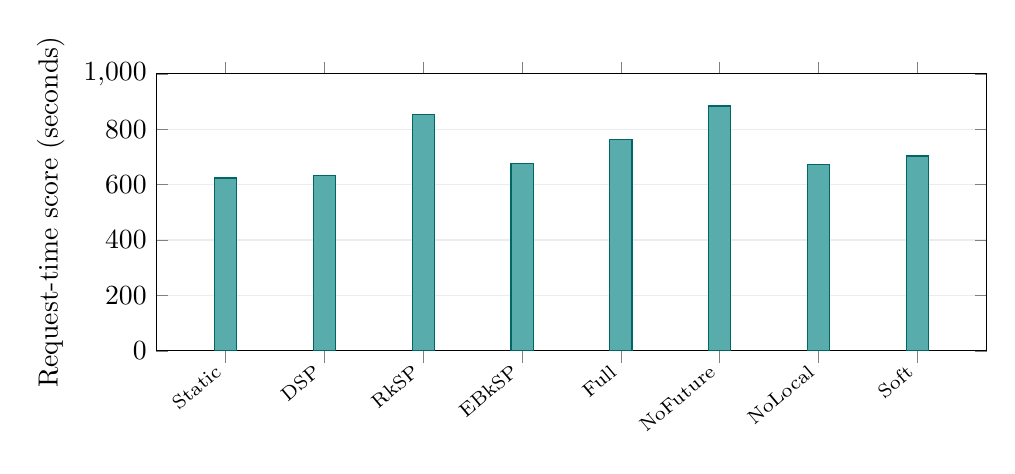
\begin{tikzpicture}
\begin{axis}[width=\columnwidth,height=5.1cm,ybar,bar width=8pt,ymin=0,ymax=1000,
 ylabel={Request-time score (seconds)},symbolic x coords={Static,DSP,RkSP,EBkSP,Full,NoFuture,NoLocal,Soft},
 xtick=data,x tick label style={rotate=40,anchor=east,font=\scriptsize},
 ymajorgrids=true,grid style={gray!15}]
\addplot[fill=teal!65,draw=teal!80!black] coordinates
 {(Static,623.984) (DSP,631.813) (RkSP,851.931) (EBkSP,677.274) (Full,762.581) (NoFuture,883.734) (NoLocal,672.136) (Soft,703.422)};
\end{axis}
\end{tikzpicture}
\caption{Microscopic execution reverses the point-queue improvement. Every policy's score includes rejected and unfinished requests. Full is original RoadFit; Soft disables only hard locality admission. Prior-art labels denote departure-policy adaptations.}
\end{figure}

The soft-locality variant assigns all requests, but 2,178 remain unfinished at the horizon. It is still worse than static by $79.44$ seconds ($[15.71,159.16]$), or 11.86\% in mean scenario-relative terms. Its difference from original RoadFit is $-59.16$ seconds with an interval spanning zero ($[-137.89,24.35]$). Removing all locality terms also restores assignment coverage but leaves unfinished trips. Thus abstention alone does not account for the failures. The controller with future scoring improves over its no-future ablation by $121.15$ seconds, yet both are worse than static. A favorable ablation does not establish an effective overall system.

All 48,000 static-policy requests arrive. Across all policies, 8,072 requests are unassigned and another 13,261 are assigned but unfinished; 163 of 640 runs fail to complete every request. There are zero recorded collision-vehicle events and zero teleports. This is simulator evidence, not a physical safety guarantee. A conditional completed-trip average can obscure the failures: original RoadFit's mean of scenario-conditional means is 601.53 seconds, below static's 623.98, while its complete-request score is substantially worse. Locality exposure must likewise retain rejected requests and distinguish planned from executed distance.

The reversal appears in both regions: original RoadFit scores 751.08 versus static 591.50 seconds in Indiranagar, and 774.08 versus 656.47 in Hebbal. The frozen candidate pool, concentrated boundary demand, forecast mismatch and uncalibrated intersections limit the interpretation. They also identify concrete requirements for any subsequent improvement: explicit queue spillback, reliable current-state estimation, and validation on fresh scenarios rather than retuning the reported seeds.

Under static routing, actuated rather than static signals reduce the score by $6.55$ seconds ($[-9.38,-3.82]$), a 1.01\% mean scenario-relative improvement. This finding contradicts a blanket claim that signal management cannot help within these test conditions. It does not evaluate a calibrated citywide signal policy or establish the best combination of route and signal control.

\subsection{Recorded travel-time prediction}
We fit histogram gradient boosting with 200 iterations, 15 leaves, learning rate $0.06$, $L_2=5$, log-time targets and seed 41. Features are route distance, origin/destination coordinates, and cyclic departure-time and weekday encodings. Parameters are fixed across feature ablations. Geometry comes from recorded trajectories, as in a supplied-path ETA task; prospective deployment assumes equivalent planned-route geometry. Models are not transferred into Bengaluru without calibration.

Table~\ref{tab:eta} shows test errors. Route and clock features improve MAE over the median-speed comparator by 1.77 minutes; the driver-cluster paired bootstrap interval is $[-2.18,-1.40]$ minutes. No exact duplicate trips cross the fitting and test files; 97 test drivers also appear in fitting, but their identities are excluded as features. A nominal 90\% absolute-residual interval has 89.43\% empirical coverage and a mean width of 21.37 minutes. That wide interval is a limitation, not an accuracy achievement. Calibration/test date shifts preclude an unqualified coverage guarantee.

\begin{table}[t]
\caption{Later-date recorded Chengdu sample: 1,400 test trips. MAE and RMSE in minutes; MAPE in percent.}
\label{tab:eta}
\centering
\begin{tabular}{lrrr}\toprule
Model & MAE & RMSE & MAPE\\\midrule
Median speed & 6.91 & 9.32 & 30.95\\
Distance linear & 6.70 & 8.60 & 32.54\\
Route + clock & 5.14 & 6.89 & 22.45\\
Without clock & 5.53 & 7.33 & 23.84\\
Without geometry & 5.85 & 7.67 & 26.43\\
Distance only (boosting) & 6.59 & 8.53 & 29.57\\\bottomrule
\end{tabular}
\end{table}



\section{Limitations and submission status}
The experiments do not validate Bengaluru ETA, actual traffic-officer outcomes, real parking occupancy, household counts, physical road safety, or route-choice compliance. A driving-only graph limits bicycle coverage. Tag merging, absent original turn-restriction relations, conditional access, missing weight limits, category radii, and terminal-neighbourhood approximations all limit admissibility. Regional boundaries exclude possible detours. The forecast model assumes an unobserved initial backlog of zero and ignores lane changes, spillback, intersection signals and heterogeneous headway interactions. SUMO includes several of these execution effects, but its generated connections and assumed signals are not surveyed Bengaluru controls. Pedestrian activity and motorcycle filtering through gaps are not calibrated.

The candidate bound is heuristic and the local admission policy can reject useful routes. Detour limits are predicted, not realized. The social term is a proxy and has no demonstrated incremental benefit in these experiments. Small regional routing gains should not be represented as solving Bengaluru congestion. The Chengdu sample establishes a separate predictive baseline, not controller effectiveness or state-of-the-art ETA performance. Source-specific raw data, requests, scripts, hashes, and manifests make these limits auditable.

Before an external high-tier research submission, the work requires a defensible contribution, full direct-prior-art and stronger neural comparisons, an independently calibrated traffic environment, partial-observation and forecast-error stress tests in the microscopic setting, and prospective or observational Bengaluru travel-time validation. The present cross-model evaluation tests failure modes rather than establishing universal superiority. Broader reproducible insights may support an experiment/benchmark paper, but acceptance cannot be inferred from code correctness or a target percentage. The current document is an internal review draft; author responsibility, venue-specific formatting, publication rights and required disclosures must be finalized by the human authors.

\section{Reproducibility and responsible presentation}
Acquisition manifests pin source repositories and hash downloaded data. Experiment manifests record seeds, controller settings, input hashes and source hashes; raw method--request tables accompany episode summaries. Scientific figures and cluster contrasts are generated from those tables. All 104 Python tests pass. An independent XML audit checks all 384,000 SUMO method--request records, and a separate replay of one 300-request scenario matches all eight policies exactly in decisions and native outcome attributes (2,400 records). This replay establishes that scenario's local reproducibility, not cross-platform bitwise equivalence of every experiment. All reported experiments use local CPU workers; graph searches, SUMO execution, fluid queues and the small gradient-boosting baseline do not require GPU training.

The prototype does not contact drivers, traffic officers or conference systems. It manipulates local research intentions and scenarios. Satellite imagery retains attribution, and OpenStreetMap-derived data retain their provenance. No nonpublic user travel records were used. The human authors must review trajectory-data permissions and institutional obligations before redistribution or further human-subject evaluation. AI assistance was used to develop code, research summaries, experiments, figures and this manuscript. It must not be listed as an author; humans must independently verify the claims and citations before submission.

\begin{thebibliography}{99}
\bibitem{pan2012} Juan (Susan) Pan, Mohammad A. Khan, Iulian Sandu Popa, Karine Zeitouni, and Cristian Borcea. 2012. Proactive Vehicle Re-routing Strategies for Congestion Avoidance. In \emph{IEEE DCOSS}, 265--272. \url{https://doi.org/10.1109/DCOSS.2012.29}.
\bibitem{reservation2018} C. Menelaou, P. Kolios, S. Timotheou, and C. G. Panayiotou. 2018. Effective Prediction of Road Segment Occupancy for the Route-Reservation Architecture. \emph{IFAC-PapersOnLine} 51(9), 470--475. \url{https://doi.org/10.1016/j.ifacol.2018.07.077}.
\bibitem{r32014} Henan Wang et al. 2014. R3: A Real-Time Route Recommendation System. \emph{PVLDB} demonstration. \url{https://www.vldb.org/2014/program/papers/demo/p1007-wang.pdf}.
\bibitem{deeptte2018} Dong Wang, Junbo Zhang, Wei Cao, Jian Li, and Yu Zheng. 2018. When Will You Arrive? Estimating Travel Time Based on Deep Neural Networks. In \emph{AAAI}. \url{https://doi.org/10.1609/aaai.v32i1.11877}.
\bibitem{heteta2020} Huiting Hong et al. 2020. HetETA: Heterogeneous Information Network Embedding for Estimating Time of Arrival. In \emph{KDD}. \url{https://www.kdd.org/kdd2020/accepted-papers/view/heteta-heterogeneous-information-network-embedding-for-estimating-time-of-a.html}.
\bibitem{bustr2020} Richard Barnes et al. 2020. BusTr: Predicting Bus Travel Times from Real-Time Traffic. In \emph{KDD}. \url{https://www.kdd.org/kdd2020/accepted-papers/view/bustr-predicting-bus-travel-times-from-real-time-traffic.html}.
\bibitem{futurelight2026} Zizhuo Xu et al. 2026. FutureLight: An Efficient Future Traffic Data-Driven Reinforcement Learning Framework for Traffic Signal Controls. Listed in the VLDB 2026 research program. \url{https://vldb.org/2026/program.html}.
\bibitem{valhalla} Valhalla contributors. Routing API reference, truck costing options. \url{https://valhalla.github.io/valhalla/api/route/api-reference/}.
\bibitem{tntp} Ben Stabler, Hillel Bar-Gera, Elizabeth Sall and contributors. Transportation Networks for Research. Dataset source and individual network documentation. \url{https://github.com/bstabler/TransportationNetworks}.
\bibitem{deepttecode} Urban Computing contributors. DeepTTE author code and sample trajectories. \url{https://github.com/UrbComp/DeepTTE}.
\bibitem{sumo2018} Pablo Alvarez Lopez et al. 2018. Microscopic Traffic Simulation using SUMO. In \emph{IEEE ITSC}, 2575--2582. \url{https://doi.org/10.1109/ITSC.2018.8569938}.
\bibitem{iocsurvey} Bengaluru Smart Infrastructure Limited and NEZ Infratech. 2025. Elevated Rotary Flyover at IOC Junction and Additional Two-Lane ROB at Baiyyappanahalli Railway Level Crossing: Detailed Project Report, Volume I. September 2025; traffic survey sheets dated 24 August 2021. OpenCity public mirror, resource identifier \texttt{bfdd8181-2bc7-49cf-8c47-a700ec59caa1}. Source URL, PDF hash, page references and transcription quality flags accompany the artifact.
\end{thebibliography}

\appendix
\section{Artifact entry points}
Run \texttt{scripts/acquire\_public\_data.py} separately for OSM and TNTP; \texttt{scripts/prepare\_bengaluru\_regions.py} extracts the six regions. \texttt{src.evaluation.traffic\_benchmark} runs public-network scenarios. \texttt{src.evaluation.bengaluru\_benchmark} accepts \texttt{all\_nodes} or \texttt{arterial} OD policies. \texttt{scripts/acquire\_eta\_sample.py} retrieves the pinned author sample; \texttt{scripts/evaluate\_eta\_sample.py} fits prediction baselines. \texttt{scripts/analyze\_traffic\_results.py} creates cluster intervals and figures. Pinned dependencies, raw tables, source/input hashes and detailed reproduction commands are supplied with the repository. Historical synthetic geometry experiments are retained separately and are not mixed with these traffic-control results.

Install the separate \texttt{requirements-sumo.txt} environment additions for microscopic evaluation. The modules \texttt{scripts.prepare\_sumo}, \texttt{src.evaluation.sumo\_benchmark}, \texttt{scripts.analyze\_sumo}, and \texttt{scripts.verify\_sumo} prepare, execute, analyze and audit the new study. Native trip records, decisions, network XML and scenario demands accompany the summary tables. The verifier recomputes completion, elapsed time including insertion delay, capped score, class permissions and route connectivity independently from the recorded XML and decisions. The manuscript source remains in its original editor; earlier review PDFs are historical snapshots and do not represent this revision.
\end{document}
